\documentclass[11pt,a4paper]{article}

% ===== Silnik: tectonic / XeTeX =====
\usepackage{fontspec}
\usepackage{polyglossia}
\setdefaultlanguage{polish}

\usepackage{amsmath}
\usepackage{amssymb}
\usepackage[a4paper,margin=2.5cm]{geometry}
\usepackage{graphicx}
\usepackage{booktabs}
\usepackage{array}
\usepackage{float}
\usepackage{xcolor}
\usepackage{enumitem}
\usepackage{caption}
\usepackage{hyperref}
\hypersetup{colorlinks=true, linkcolor=blue!45!black, urlcolor=blue!45!black, citecolor=blue!45!black}

\captionsetup{font=small, labelfont=bf}
\graphicspath{{figures/}}
\setlength{\parskip}{0.5em}
\setlength{\parindent}{0pt}

\title{\textbf{Sprawozdanie z projektu}\\[0.4em]
\large Ewolucja ekosystemów języków programowania na GitHubie (2011--2026)}
\author{Mateusz Lampert, Wojciech Maćkowiak\\[0.4em]
Projekt UMISI --- Grupa 1 (projekty dziedzinowe i aplikacyjne)\\
Temat 5: Ewolucja ekosystemów języków programowania}
\date{\today}

\begin{document}

\maketitle

\begin{abstract}
\noindent
Projekt analizuje zmiany popularności 21 głównych języków programowania na podstawie
aktywności typu \texttt{PushEvent} w publicznych repozytoriach GitHub w latach
2011--2026 (dane z GH~Archive eksportowane przez BigQuery). Celem jest pokazanie
trendów popularności w czasie, porównanie aktywności społeczności oraz wykrycie
struktury podobieństwa ekosystemów językowych. Zbudowano kompletny potok przetwarzania
danych w~Pythonie (ETL $\rightarrow$ budowa wektorów cech $\rightarrow$ redukcja wymiaru
$\rightarrow$ EDA $\rightarrow$ generowanie wizualizacji) oraz interaktywny dashboard
(\texttt{index.html}) oparty na Vega-Lite i~Plotly. Wektory profili czasowych poddano
siedmiu metodom redukcji wymiaru (PCA, kernel~PCA, t-SNE, UMAP, TriMAP, PaCMAP, OpenTSNE)
w~2D i~3D oraz klastrowaniu metodą $k$-średnich. Sprawozdanie omawia źródło i~preprocessing
danych, architekturę rozwiązania, wyniki analizy oraz ich ostrożną interpretację.
\end{abstract}

\tableofcontents
\newpage

% ============================================================
\section{Cel i zakres projektu}

Projekt realizuje temat~5 z~Grupy~1 zajęć UMISI --- \emph{Ewolucja ekosystemów języków
programowania}. Grupa~1 obejmuje projekty dziedzinowe i~aplikacyjne oparte na dużych
zbiorach danych, których wspólnym elementem jest przygotowanie reprezentacji
wielowymiarowych, zastosowanie metod redukcji wymiaru, wizualizacja struktur w~przestrzeni
2D oraz --- często --- klastrowanie i~wykrywanie obserwacji nietypowych.

\textbf{Cel projektu:} pokazanie zmian popularności języków programowania i~technologii
w~czasie na podstawie danych o~aktywności w~repozytoriach GitHub.

\textbf{Zakres:}
\begin{itemize}[nosep]
  \item przygotowanie danych o~aktywności repozytoriów per język,
  \item analiza popularności języków w~czasie,
  \item porównanie aktywności społeczności kontrybutorów,
  \item interaktywne wykresy trendów,
  \item analiza zmian dominujących technologii i~koncentracji rynku,
  \item element redukcji wymiaru: budowa wektorów profili czasowych i~porównanie wyników
        wielu metod (m.in. UMAP, TriMAP, PaCMAP),
  \item interpretacja wyników.
\end{itemize}

Analizą objęto \textbf{21 najpopularniejszych języków} (wg aktywności \texttt{PushEvent}):
JavaScript, Python, Java, TypeScript, C\#, C++, PHP, C, Go, Ruby, Rust, Kotlin, Swift,
Dart, Scala, R, Objective-C, Lua, Haskell, Julia, Perl. Horyzont czasowy obejmuje okres
od początku GH~Archive (2011) do ostatniego kwartału w~danych (\textbf{2026-04-01}, tj. Q2~2026).

% ============================================================
\section{Dane i ich pozyskanie}

\subsection{Źródło danych}

Dane pochodzą z~\textbf{dwóch publicznych zbiorów dostępnych w~Google BigQuery}, które
zostały \textbf{złączone po repozytorium} (zapytanie \texttt{sql/bigquery\_export.sql}):

\begin{enumerate}[leftmargin=1.5em]
  \item \textbf{GH~Archive} (\texttt{githubarchive.day.20*}) --- strumień \emph{zdarzeń}
        GitHub. Z~niego pobieramy \textbf{aktywność}: zdarzenia \texttt{PushEvent} (commity)
        oraz \texttt{actor.id} (kto pushował) wraz z~identyfikatorem repozytorium, do którego
        trafił push. To jest źródło ,,ile się działo'' --- liczba commitów i~unikalnych aktorów
        w~czasie.
  \item \textbf{GitHub Repos} (\texttt{bigquery-public-data.github\_repos.languages}) ---
        snapshot \emph{zawartości} repozytoriów. Z~niego pobieramy \textbf{skład językowy} każdego
        repo: dla każdego języka liczbę bajtów kodu (\texttt{lang.name}, \texttt{lang.bytes}).
        To jest źródło ,,z~czego repo jest zbudowane'' --- na jakie języki dany commit
        ,,wędruje''.
\end{enumerate}

\textbf{Idea złączenia.} Sam strumień zdarzeń nie mówi, w~jakim języku napisano commit ---
mówi tylko, do którego repozytorium trafił. Dlatego dla każdego repozytorium liczymy z~drugiego
zbioru \emph{wagi językowe} (\texttt{lang\_fraction} $=$ \texttt{bytes(język)/suma\_bytes(repo)}),
a~następnie każdemu \texttt{PushEvent} przypisujemy języki repozytorium proporcjonalnie do tych
wag. Złączenie odbywa się po znormalizowanym ,,slugu'' repozytorium (\texttt{właściciel/nazwa}).
W~efekcie jeden push do repo zbudowanego np.\ w~55\% z~C++ i~45\% z~C dokłada $0{,}55$ do licznika
C++ i~$0{,}45$ do licznika C.

Eksportowany plik CSV (wynik zapytania) ma następujący schemat:

\begin{center}
\begin{tabular}{@{}lp{11cm}@{}}
\toprule
\textbf{Kolumna} & \textbf{Znaczenie} \\
\midrule
\texttt{month} / \texttt{quarter} & oś czasu (miesiąc \texttt{YYYY-MM} albo pierwszy dzień kwartału \texttt{YYYY-MM-DD}) \\
\texttt{language} & nazwa języka ze~snapshotu \texttt{github\_repos.languages} \\
\texttt{push\_events} & suma wag \texttt{lang\_fraction} po wszystkich pushach w~okresie (,,push-równoważne'' ułamki; wartość niecałkowita) \\
\texttt{unique\_actors} & liczba unikalnych \texttt{actor.id} (z~GH~Archive) \\
\bottomrule
\end{tabular}
\end{center}

\textbf{Charakter metryki.} Kolumna \texttt{push\_events} to \emph{ważona} aktywność
(suma ułamków bajtowych), a~nie ,,goła liczba \texttt{PushEvent}''. Dzięki temu jest spójna
z~udziałami procentowymi i~koncentracją rynku, ale jej \emph{absolutna skala} zależy od definicji
wag oraz od kompletności obu zbiorów --- w~szczególności od tego, dla ilu repozytoriów istnieje
snapshot składu językowego (repo bez wpisu w~\texttt{github\_repos.languages} nie wnosi wag).

\subsection{Preprocessing (ETL)}

Potok \texttt{src/etl.py}:
\begin{enumerate}[nosep]
  \item filtrowanie do 21 wybranych języków,
  \item obliczenie udziałów w~każdym okresie (\texttt{share\_pct}),
  \item metryki społeczności: unikalni aktorzy, intensywność \texttt{events\_per\_actor}, ranking,
  \item koncentracja rynku: indeks HHI oraz udział trzech liderów (top~3).
\end{enumerate}

\textbf{Luka czasowa 2013--2014.} Surowy eksport BigQuery (\texttt{manyLanguages.csv}) bywa
niespójny --- np. skok z~2012 do~2015. Aby wykresy nie miały dziury czasowej, brakujące
kwartały uzupełniono \textbf{interpolacją liniową} skryptem
\texttt{src/interpolate\_quarter\_gaps.py}; domyślnym wejściem ETL jest plik wynikowy
\texttt{data/raw/real/manyLanguages\_added.csv}. Dostępny jest też tryb syntetyczny
(\texttt{UMISI\_USE\_FAKE\_SAMPLE=1}) generujący dane miesięczne do testów potoku.

Pliki pośrednie (\texttt{data/processed/}) obejmują m.in. \texttt{monthly\_activity.csv},
\texttt{monthly\_shares.csv}, \texttt{community\_metrics.csv},
\texttt{market\_concentration.csv}, \texttt{language\_vectors.csv},
\texttt{dim\_reduction.csv} / \texttt{dim\_reduction\_3d.csv},
\texttt{language\_profiles.csv}, \texttt{language\_clusters.csv} oraz
\texttt{pca\_explained\_variance.csv}.

% ============================================================
\section{Architektura rozwiązania}

Projekt nie przechowuje gotowych wykresów jako jedynego źródła prawdy --- \textbf{wizualizacje
są generowane skryptami} z~plików CSV. Uruchomienie \texttt{python src/run\_pipeline.py}
wykonuje kolejne kroki potoku i~składa dashboard \texttt{index.html}.

\begin{center}
\begin{tabular}{@{}clp{9.5cm}@{}}
\toprule
\textbf{Krok} & \textbf{Skrypt} & \textbf{Zadanie} \\
\midrule
1 & \texttt{generate\_sample\_data.py} & (opcjonalnie) dane syntetyczne, gdy \texttt{UMISI\_USE\_FAKE\_SAMPLE=1} \\
2 & \texttt{etl.py} & wczytanie i~filtrowanie danych, udziały, metryki, koncentracja \\
3 & \texttt{build\_vectors.py} & długi format wektorów cech (profil czasowy języka) \\
4 & \texttt{dim\_reduction.py} & 7 metod redukcji wymiaru w~2D i~3D \\
5 & \texttt{eda.py} & statystyki per język, klastry $k$-means, wariancja PCA, profile \\
6 & \texttt{build\_viz.py} & główny generator: Altair $\rightarrow$ Vega-Lite, Plotly 3D, montaż \texttt{index.html} \\
7 & \texttt{build\_yearly\_viewer.py} & strona rocznego podglądu (treemap / siatka) \\
8 & \texttt{build\_market\_snapshot\_viewer.py} & strona mapy udziałów (kwartalna) \\
9 & \texttt{build\_concentration\_viewer.py} & strona koncentracji rynku \\
\bottomrule
\end{tabular}
\end{center}

\subsection{Reprezentacja wielowymiarowa i transformacja cech}

Z~tabeli udziałów budowana jest macierz profili: \textbf{wiersze = języki},
\textbf{kolumny = kolejne okresy} (pivot \texttt{share\_pct}, braki $\rightarrow 0$).
Na macierz nakładana jest transformacja \texttt{share\_pct} $\rightarrow$ \texttt{log1p}
$\rightarrow$ \texttt{StandardScaler} (standaryzacja \emph{per kolumna}, czyli per okres
czasu). Wynik to macierz o~wymiarach \textbf{21 $\times$ T}, gdzie $T$ to liczba unikalnych
okresów (w~bieżącym eksporcie $T = 62$ kwartały). Każdy wiersz to jeden język jako punkt
w~przestrzeni $\mathbb{R}^{T}$ --- to wejście do redukcji wymiaru, PCA i~klastrowania.

\subsection{Warstwa wizualizacji (dashboard)}

Dashboard \texttt{index.html} łączy:
\begin{itemize}[nosep]
  \item \textbf{wykresy Vega-Lite} (\texttt{*.vl.json}) renderowane przez \texttt{vega-embed} --- interaktywne (tooltipy, zoom);
  \item \textbf{scenę 3D Plotly} osadzoną bezpośrednio w~stronie (działa również przy otwarciu z~dysku, \texttt{file://});
  \item \textbf{trzy strony-,,viewery''} (roczny treemap, mapa udziałów, koncentracja) ładowane w~\texttt{iframe} z~animacją w~czasie.
\end{itemize}

Zakładki dashboardu: trendy aktywności, udziały w~czasie, mapa udziałów, przegląd kwartalny
treemap, koncentracja rynku, porównanie społeczności, EDA (zmiana udziału, wariancja PCA,
klastrowanie) oraz redukcja wymiaru 2D i~3D.

% ============================================================
\section{Wyniki analizy}

\subsection{Trendy aktywności w czasie}

Wykres trendów (rys.~\ref{fig:trends}) pokazuje sumę kwartalną ważonych ,,push-równoważnych''
zdarzeń per język. Widoczny jest ogólny wzrost aktywności po~ok.~2015, szczyt w~latach
\textbf{2021--2023} oraz spadek po~2023. JavaScript i~Python utrzymują wysokie poziomy,
TypeScript wyraźnie rośnie.

\begin{figure}[H]
  \centering
  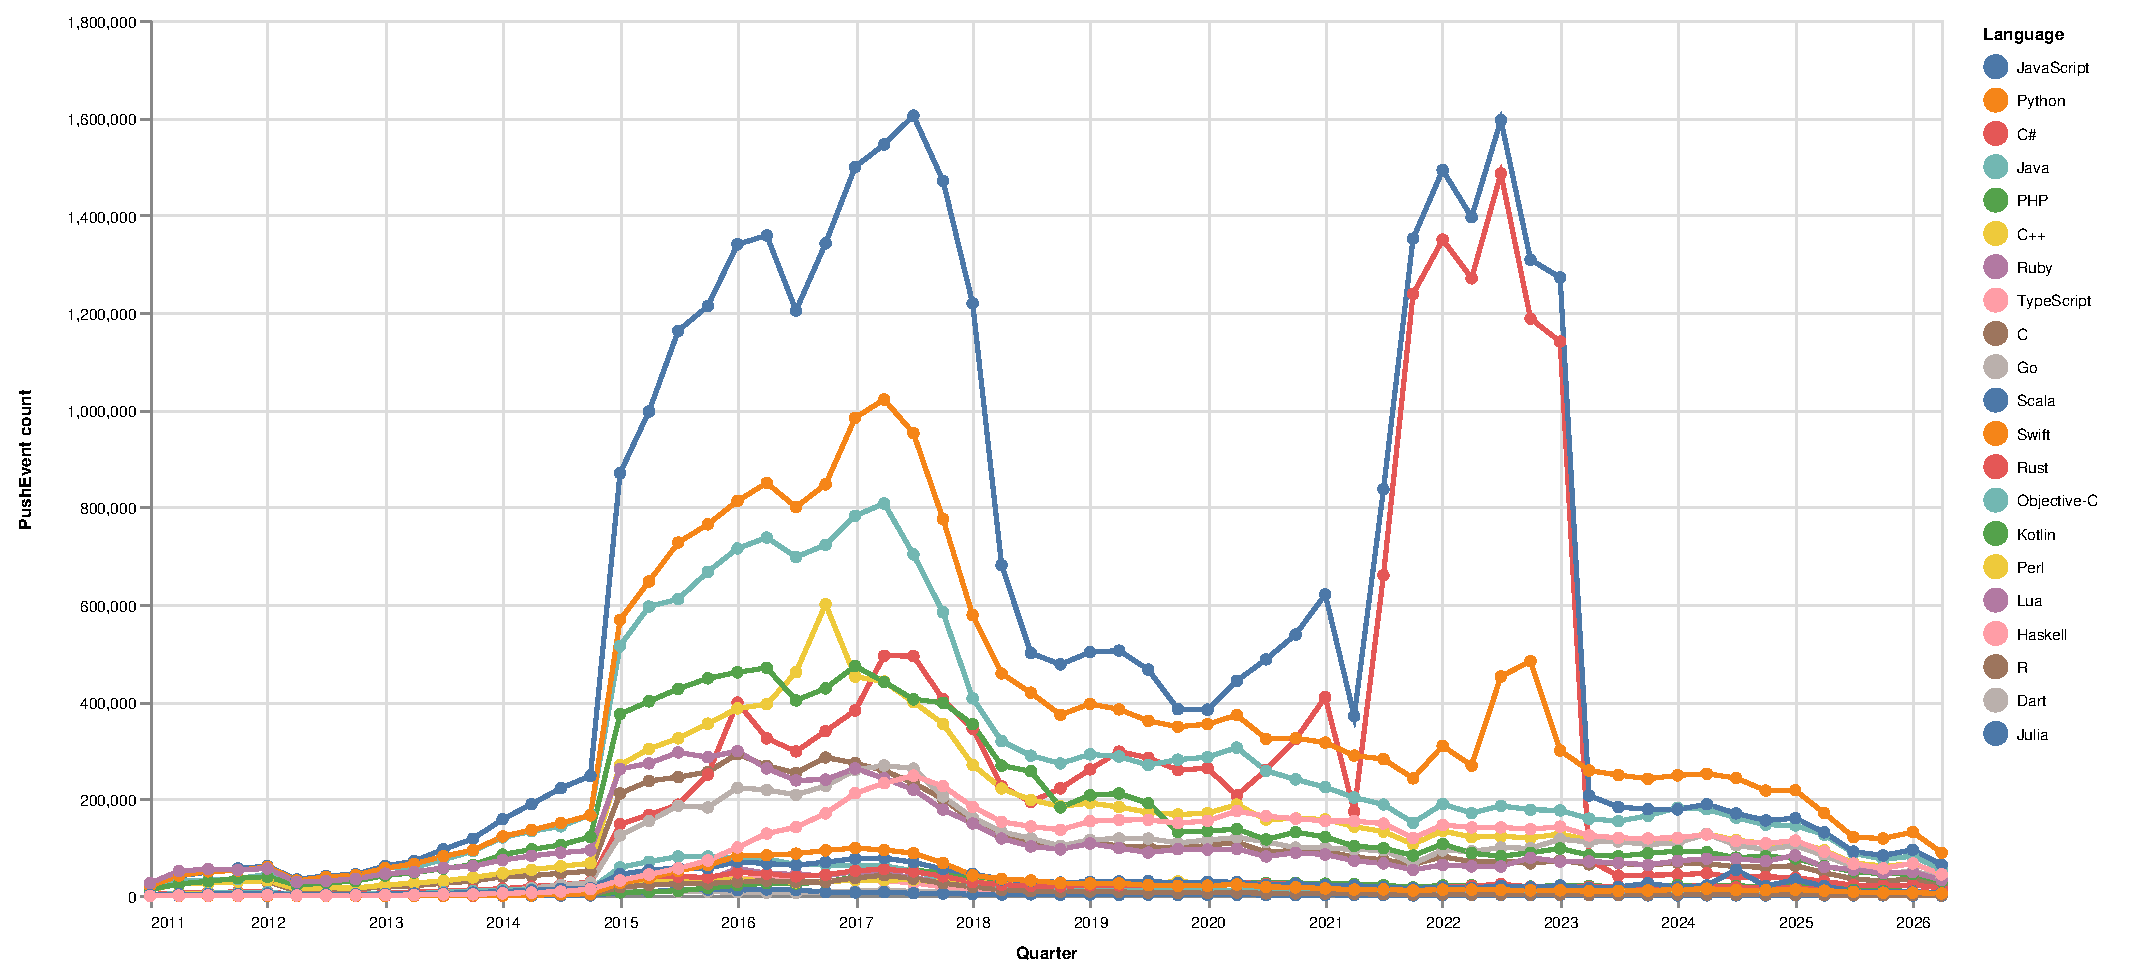
\includegraphics[width=\linewidth]{trends_line.pdf}
  \caption{Trendy aktywności: liczba (ważonych) zdarzeń \texttt{PushEvent} per język w~funkcji kwartału (2011--2026).}
  \label{fig:trends}
\end{figure}

\subsection{Mapa udziałów rynku}

Mapa udziałów (rys.~\ref{fig:market}) przedstawia procentowy udział języków w~aktywności
w~ostatnim dostępnym kwartale (Q2~2026). Dominują Python (18{,}7\%), JavaScript (13{,}5\%)
oraz Java (11{,}4\%); dalej C++, TypeScript i~Go. Widać charakterystyczny ,,długi ogon''
języków niszowych (R, Julia, Lua) o~udziałach poniżej~1\%.

\begin{figure}[H]
  \centering
  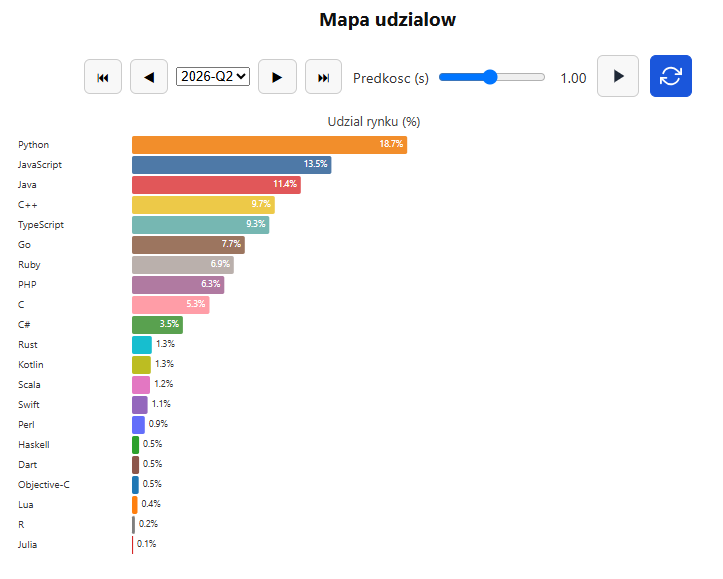
\includegraphics[width=0.82\linewidth]{market_snapshot.png}
  \caption{Mapa udziałów rynku (\%) w~kwartale Q2~2026 --- interaktywny widok z~osią czasu (animacja kwartał po kwartale).}
  \label{fig:market}
\end{figure}

\subsection{Przegląd kwartalny --- treemap}

Treemap (rys.~\ref{fig:treemap}) reprezentuje wielkość ekosystemu jako pole prostokąta
(analogia ,,mapy giełdy''). Widok jest animowany w~czasie; zrzut pokazuje wczesny okres
(Q1~2011), gdy strukturę rynku tworzyły jeszcze JavaScript, Java, Ruby, PHP, C i~Python ---
przed późniejszą ekspansją TypeScriptu, Go czy Rusta.

\begin{figure}[H]
  \centering
  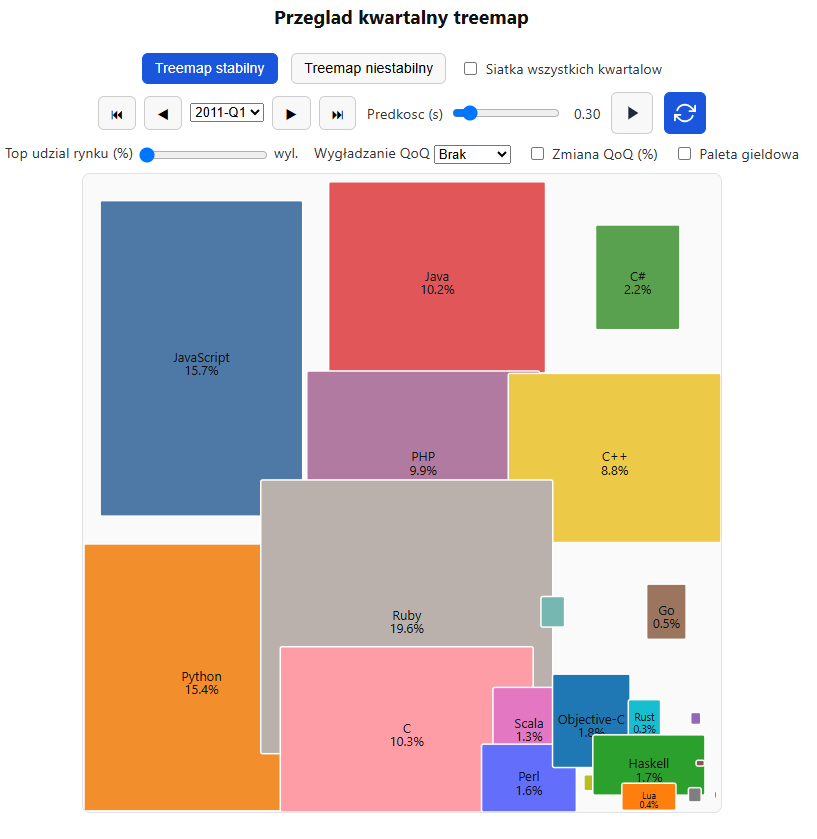
\includegraphics[width=0.74\linewidth]{treemap.png}
  \caption{Przegląd kwartalny (treemap) struktury udziałów --- stan dla Q1~2011.}
  \label{fig:treemap}
\end{figure}

\subsection{Udziały języków w czasie}

Rysunek~\ref{fig:shares} przedstawia skumulowany wykres obszarowy (\emph{stacked area})
udziałów poszczególnych języków w~całkowitej aktywności w~kolejnych kwartałach. W~przeciwieństwie
do trendów absolutnych ten widok eksponuje \emph{względną} popularność: dobrze widać stopniowe
,,kurczenie się'' udziału JavaScriptu, ekspansję Pythona i~TypeScriptu oraz erozję udziału
Ruby i~PHP, mimo że bezwzględne wolumeny rosną dla większości ekosystemów.

\begin{figure}[H]
  \centering
  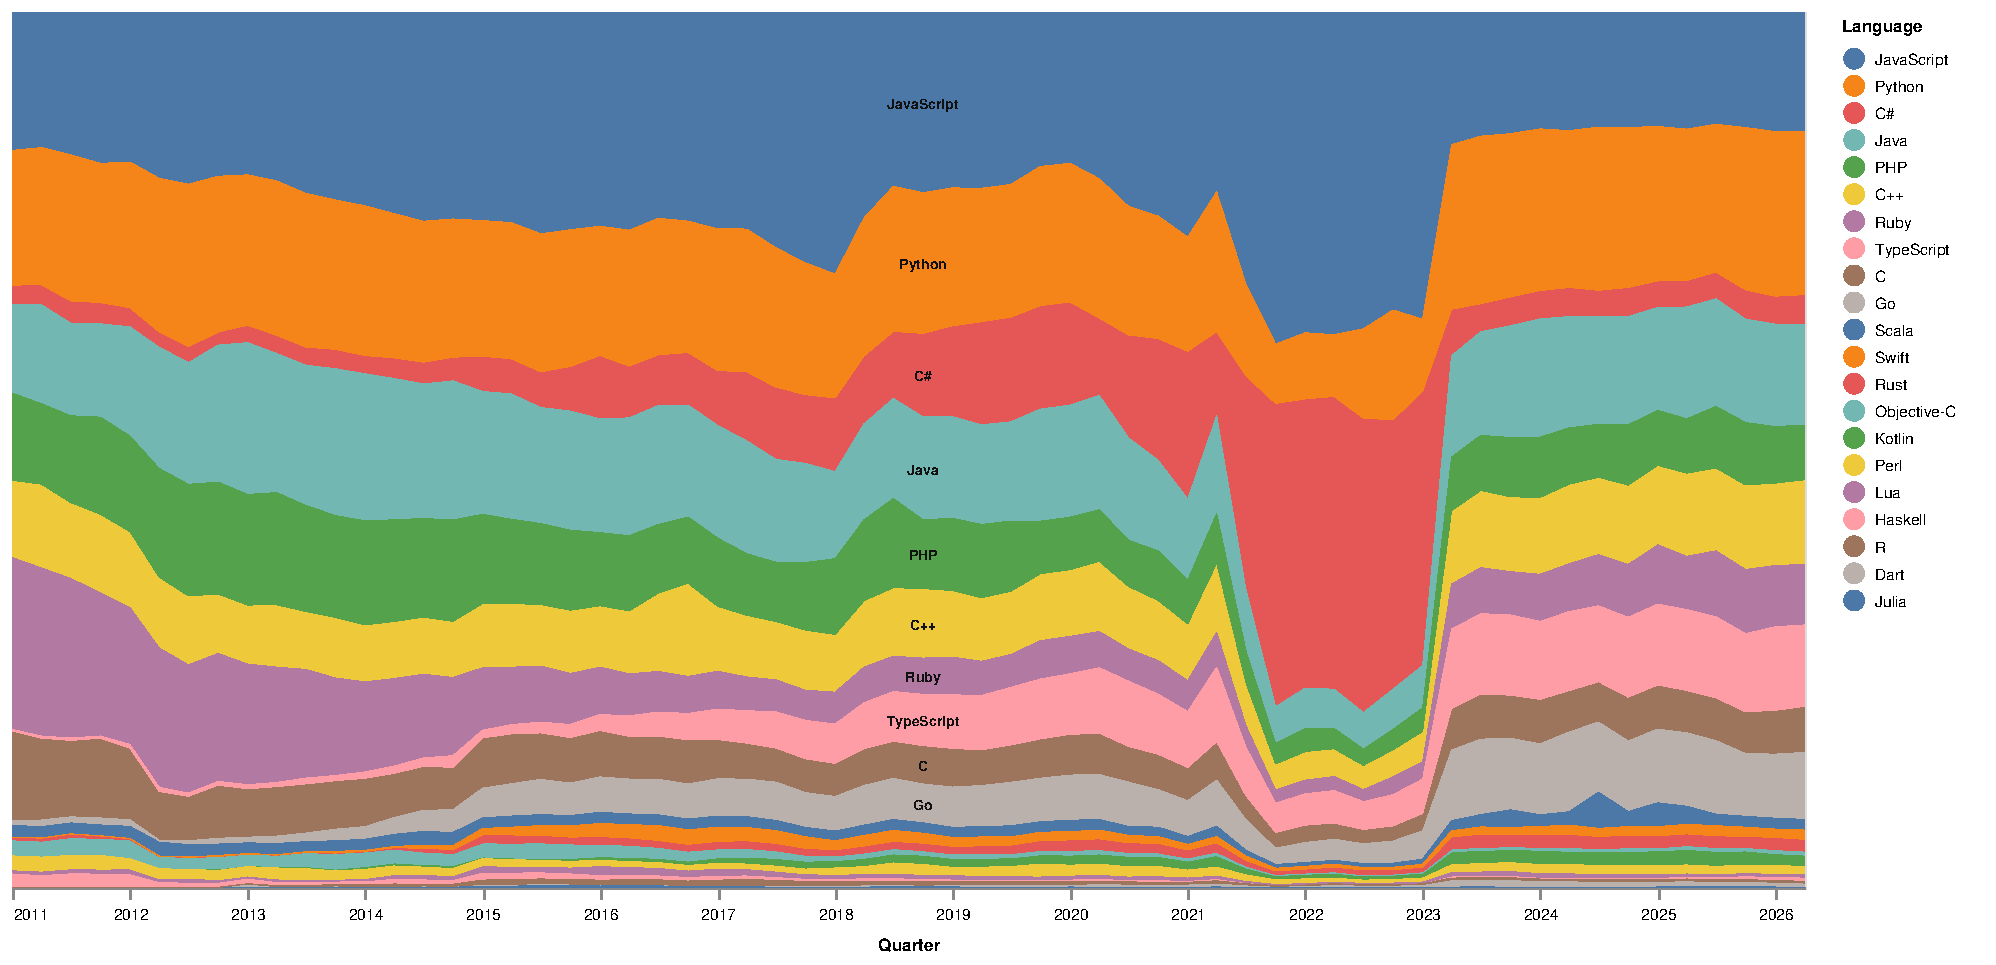
\includegraphics[width=\linewidth]{shares_stacked.pdf}
  \caption{Udziały języków w~aktywności w~czasie (skumulowany wykres obszarowy, 2011--2026).}
  \label{fig:shares}
\end{figure}

\subsection{Aktywność społeczności}

\paragraph{Porównanie społeczności.} Wykres (rys.~\ref{fig:community}) łączy dwa kanały:
słupki = suma \texttt{unique\_actors} dla top~12 języków (szerokość bazy kontrybutorów),
czarna linia = średnia \texttt{events\_per\_actor} (intensywność). Wzrost linii przy
stabilnych słupkach sugeruje wzrost intensywności (więcej zdarzeń na aktora), a nie samej
liczby osób. Należy pamiętać, że ta sama osoba kontrybuująca w~kilku językach jest liczona
wielokrotnie --- suma słupków \emph{nie} jest globalnym ,,headcountem''.

\begin{figure}[H]
  \centering
  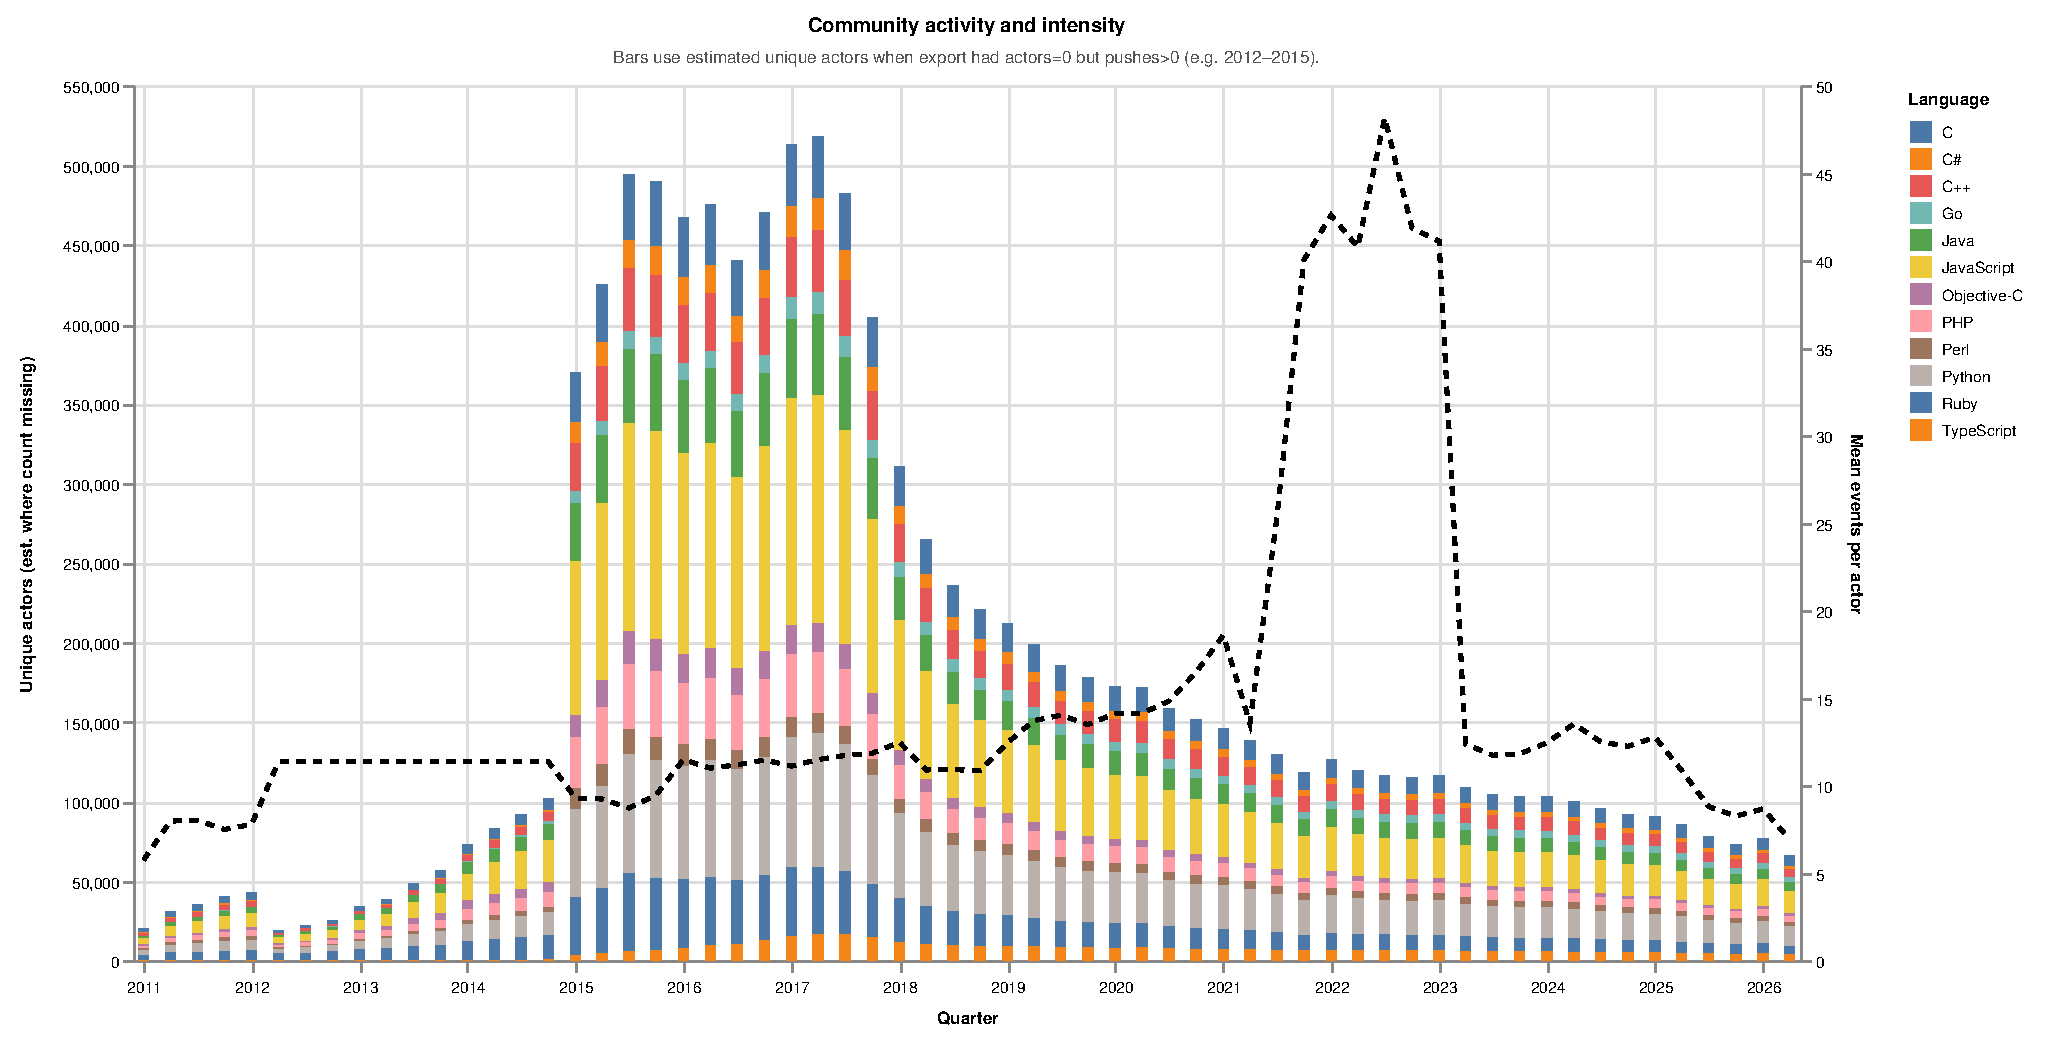
\includegraphics[width=\linewidth]{community_comparison.pdf}
  \caption{Porównanie społeczności: szerokość bazy aktorów (słupki) vs.\ średnia intensywność zdarzeń na aktora (linia).}
  \label{fig:community}
\end{figure}

% ============================================================
\section{Analiza eksploracyjna (EDA)}

\subsection{Zmiana udziału i obserwacje nietypowe}

Dla każdego języka policzono zmianę udziału (pierwszy vs.\ ostatni rok, w~punktach
procentowych) oraz nachylenie trendu (regresja liniowa). Obserwacje nietypowe (outliery)
wykrywano z~$z$-score zmienności i~zmiany udziału, próg $|z| > 1{,}5$. Rysunek~\ref{fig:share}
pokazuje, że największe \emph{wzrosty} dotyczą TypeScriptu, Go i~Pythona, a~największe
\emph{spadki} --- m.in. starszych ekosystemów; Ruby i~PHP tracą udział, podczas gdy Rust
rośnie z~niskiej bazy (typowy profil ,,emerging language'').

\begin{figure}[H]
  \centering
  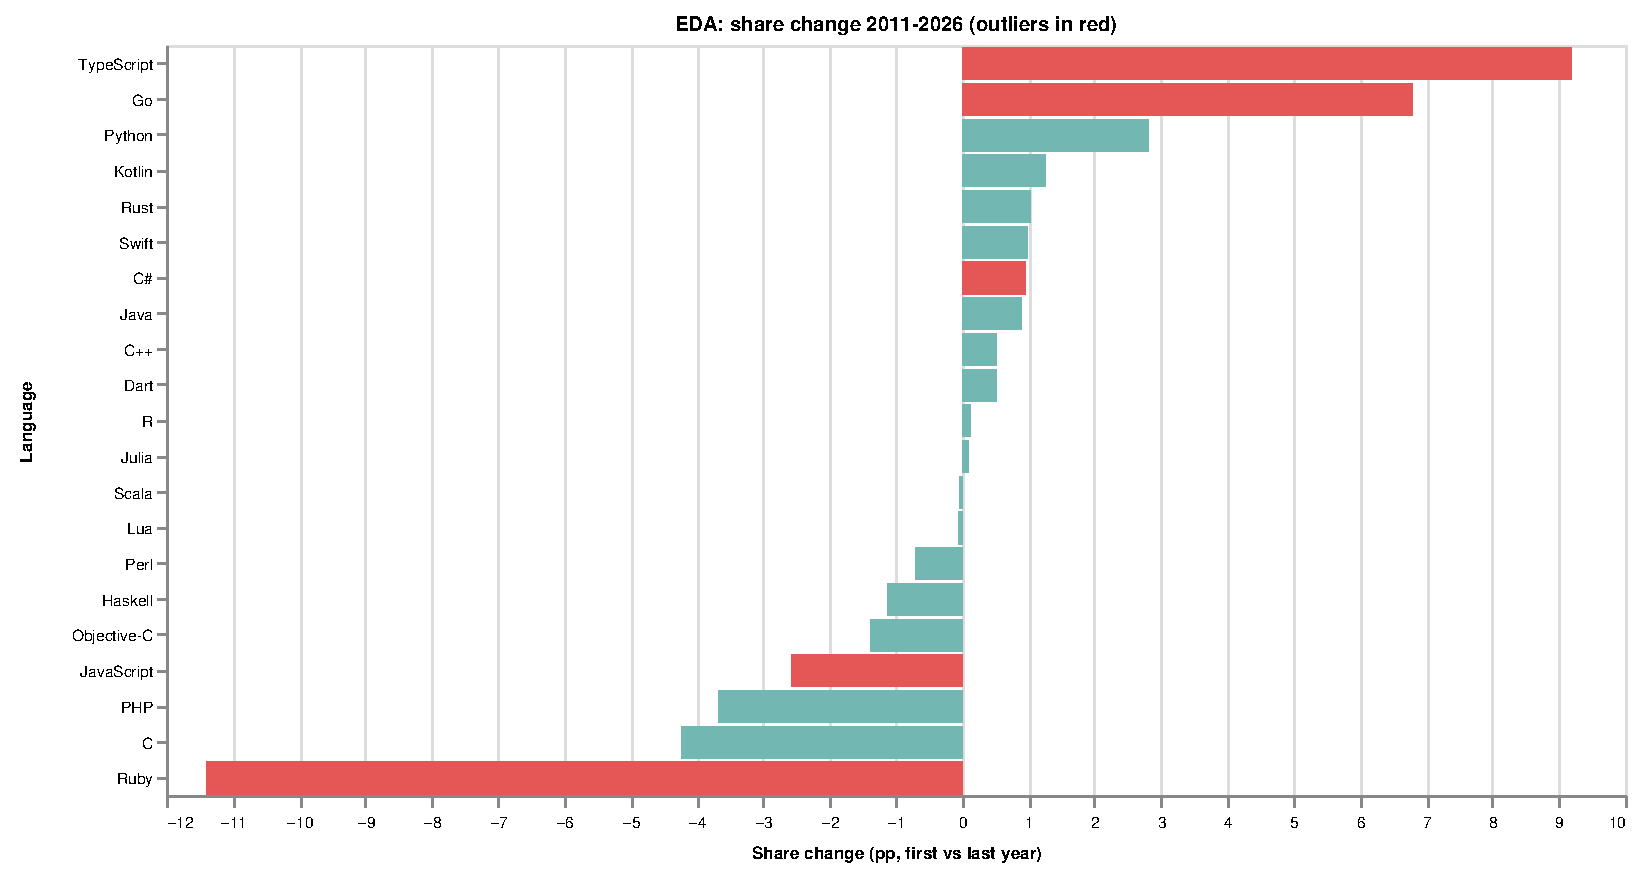
\includegraphics[width=0.9\linewidth]{share_change.pdf}
  \caption{Zmiana udziału w~aktywności (pp, pierwszy vs.\ ostatni rok). Wartości dodatnie = wzrost popularności.}
  \label{fig:share}
\end{figure}

\subsection{Klastrowanie}

Na znormalizowanych wektorach profili czasowych ($21 \times T$) zastosowano \textbf{$k$-means}
($k=3$, \texttt{random\_state}=42). Punkty na rys.~\ref{fig:clusters} są umieszczone
w~przestrzeni dwóch pierwszych składowych PCA, a~kolor oznacza przypisanie do klastra.
Wyłaniają się trzy grupy: \emph{(i)} duże, dominujące ekosystemy (JavaScript, Python, Java),
\emph{(ii)} szeroka grupa języków średnich i~niszowych oraz \emph{(iii)} ekosystemy
o~specyficznym profilu zmienności (m.in. Ruby, PHP, C, C++).

\begin{figure}[H]
  \centering
  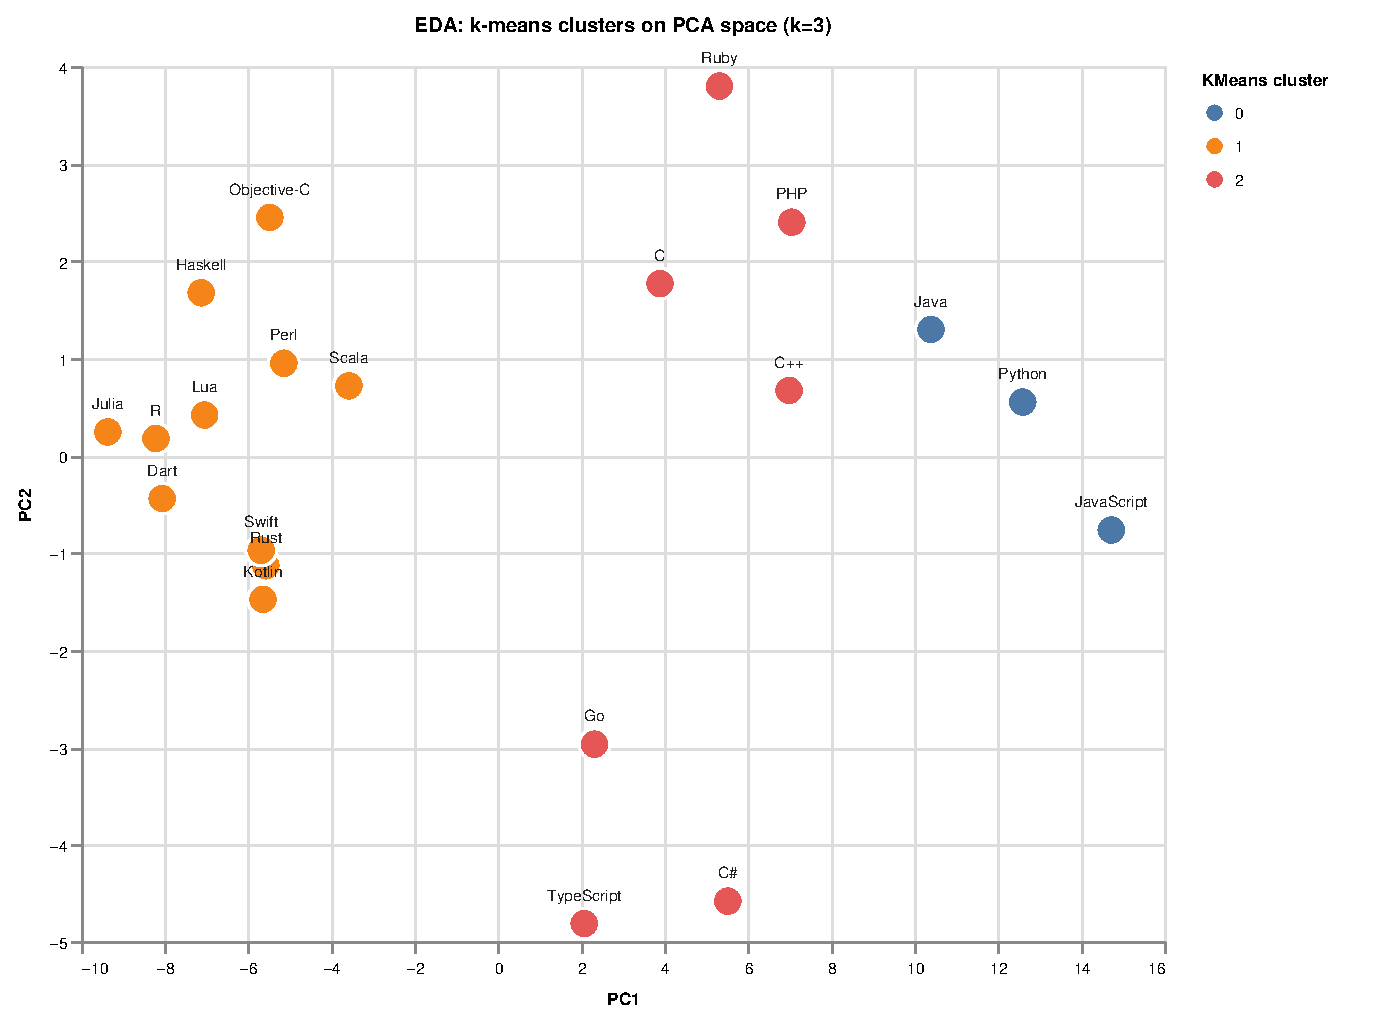
\includegraphics[width=0.95\linewidth]{clusters.pdf}
  \caption{Klastrowanie $k$-means ($k=3$) na profilach czasowych, rzutowane na płaszczyznę PC1--PC2.}
  \label{fig:clusters}
\end{figure}

% ============================================================
\section{Redukcja wymiaru}

Wektory profili czasowych (każdy język = punkt w~$\mathbb{R}^{T}$, $T=62$) zrzutowano na~2D
siedmioma metodami omawianymi na zajęciach. Każda metoda kładzie nacisk na inną własność
struktury danych:

\begin{center}
\begin{tabular}{@{}lp{10.5cm}@{}}
\toprule
\textbf{Metoda} & \textbf{Charakterystyka} \\
\midrule
PCA            & liniowa baza --- dominujące kierunki zmian w~czasie \\
Kernel PCA (RBF)& nieliniowe odwzorowanie w~przestrzeń cech, potem 2D \\
t-SNE (sklearn) & klasyczny t-SNE (Barnes--Hut) --- lokalne sąsiedztwa \\
UMAP           & zachowanie struktury lokalnej i~części globalnej \\
TriMAP         & nacisk na zachowanie tripletów odległości \\
PaCMAP         & balans bliskich i~dalekich par --- czytelna separacja klastrów \\
OpenTSNE       & szybki t-SNE (optymalizacja bliska FIt-SNE) \\
\bottomrule
\end{tabular}
\end{center}

Rysunek~\ref{fig:dimred} zestawia wszystkie siedem paneli. Panele mają \textbf{niezależne osie}
(\texttt{resolve\_scale}), więc nie porównujemy liczbowo współrzędnych między metodami ---
istotne są \emph{względne sąsiedztwa} w~obrębie jednego panelu. We wszystkich metodach języki
rosnące (TypeScript, Rust, Python) wyraźnie odróżniają się od spadających (Ruby, PHP),
a~ekosystemy enterprise (Java, C\#) lokują się pośrodku. Dodatkowo dashboard udostępnia
interaktywną \textbf{scenę 3D} (Plotly) z~tymi samymi metodami.

\begin{figure}[H]
  \centering
  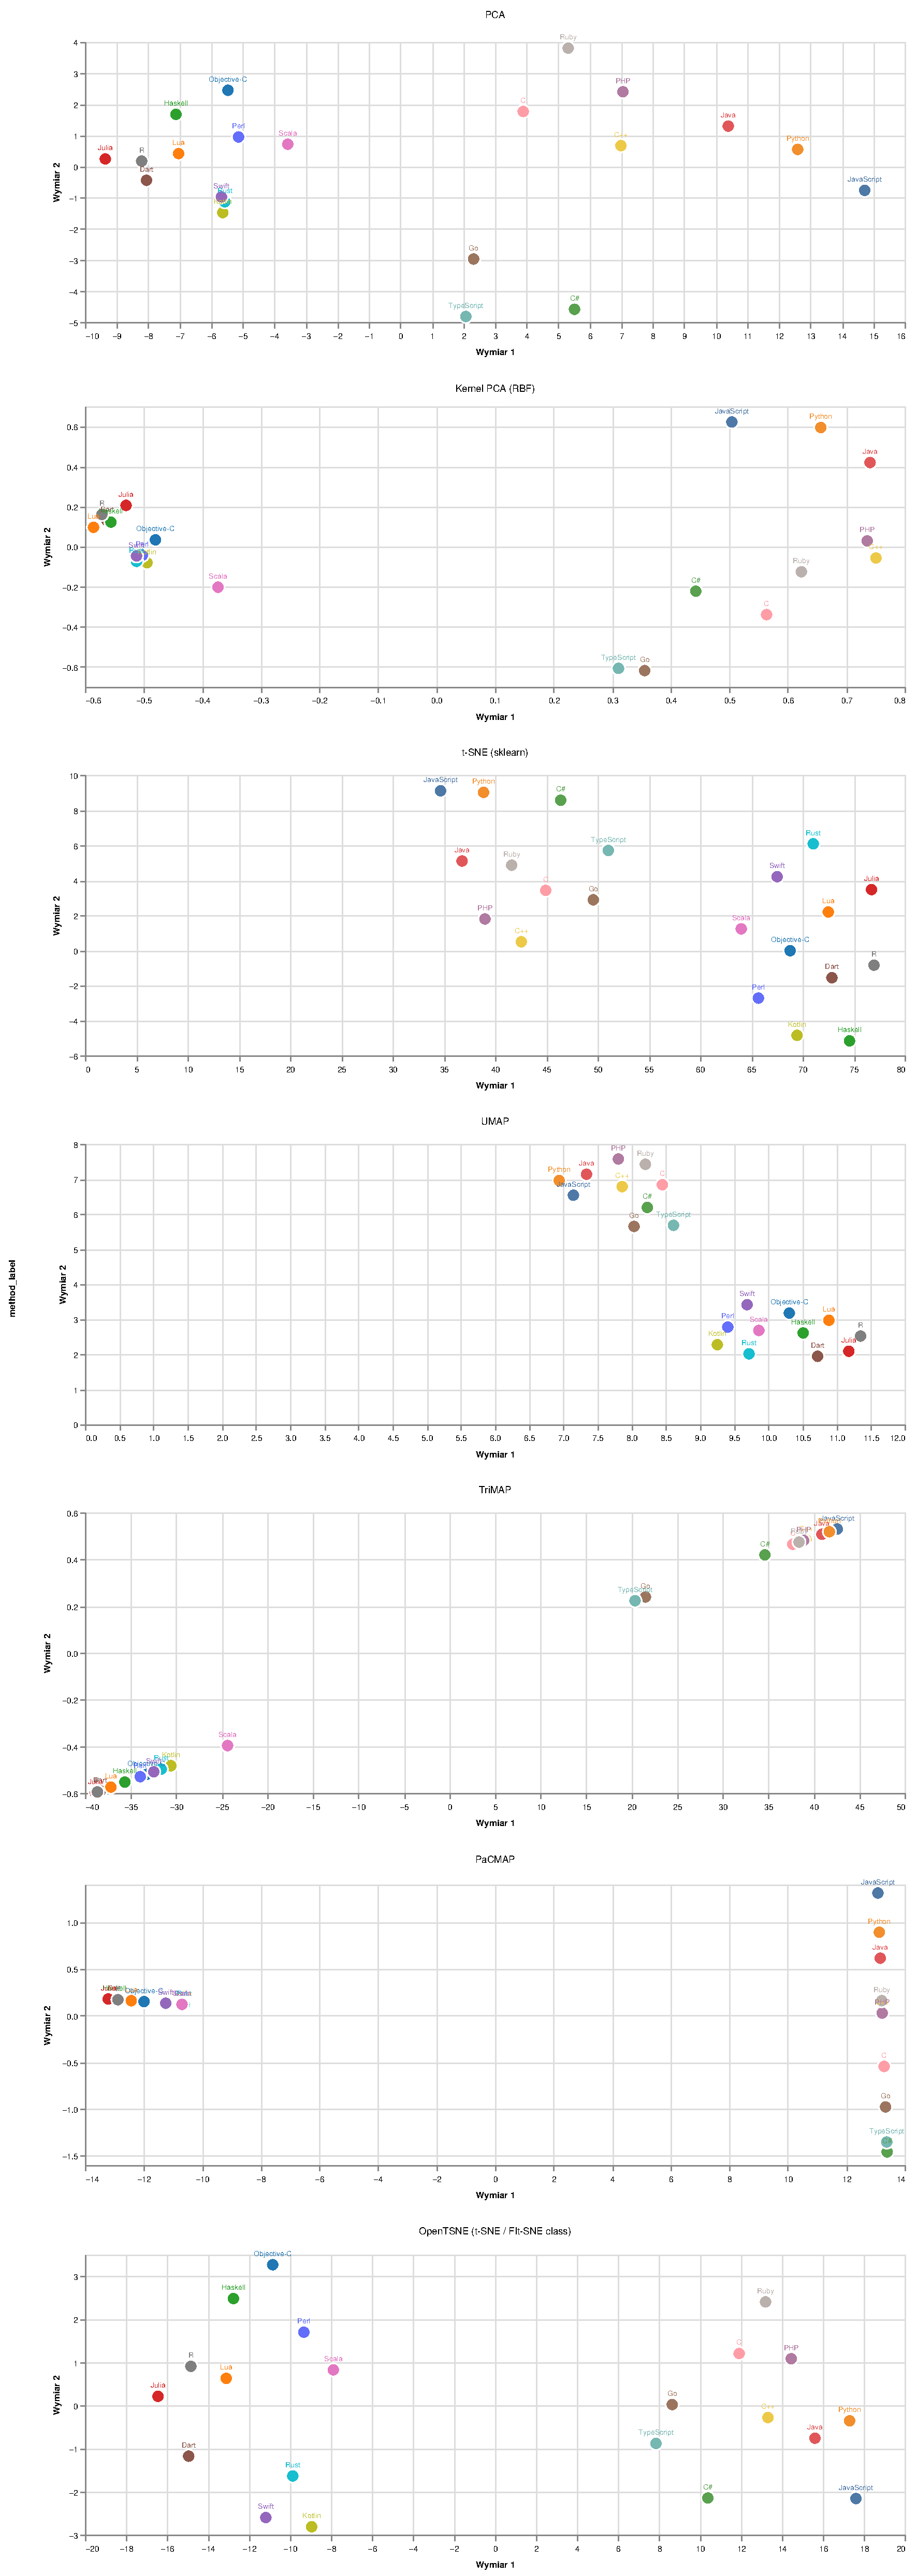
\includegraphics[height=0.86\textheight]{dim_reduction.pdf}
  \caption{Redukcja wymiaru --- 2D rzuty profili językowych siedmioma metodami (PCA, kernel~PCA, t-SNE, UMAP, TriMAP, PaCMAP, OpenTSNE). Etykiety na punktach; osie niezależne między panelami.}
  \label{fig:dimred}
\end{figure}

% ============================================================
\section{Interpretacja i wnioski}

\begin{itemize}[leftmargin=1.3em]
  \item \textbf{JavaScript} pozostaje liderem aktywności, ale jego \emph{udział} stopniowo maleje
        wraz z~różnicowaniem ekosystemu.
  \item \textbf{Python} i~\textbf{TypeScript} wyraźnie zyskują --- Python dzięki data/ML i~DevOps,
        TypeScript dzięki adopcji we frontendzie i~full-stacku.
  \item \textbf{Rust} rośnie z~niskiej bazy; \textbf{Ruby} i~\textbf{PHP} tracą udział.
  \item Rynek pozostaje \textbf{skoncentrowany} --- kilka języków dominuje (wysoki HHI, duży udział top~3).
\end{itemize}

\paragraph{Ostrożna interpretacja skoków.} Wzrost ,,wszystkiego'' po~ok.~2015 częściowo
odzwierciedla realną dynamikę (rosnąca baza publicznego kodu), a~częściowo \emph{kontekst danych}
(niespójność starszej części GH~Archive, łączenie eksportów, interpolacja luk). Szczyt
\textbf{2021--2023} \emph{nie pokrywa się} z~pierwszym lockdownem 2020 --- COVID jest tylko jednym
z~elementów tła. Bardziej wiarygodna jest narracja \textbf{wieloczynnikowa}: opóźniona reakcja
gospodarki, druga fala cyfryzacji (remote, cloud), fale hype'u (web3/NFT, boom ML/AI), produkty
GitHub (np.\ Copilot od~2021) oraz aktywność botów/CI. Spadek po~2023 może wynikać z~normalizacji
po~przegrzaniu, redukcji zatrudnienia w~tech oraz przesunięcia pracy do~repozytoriów prywatnych
(których archiwum \emph{nie} widzi). Zaleca się rozdzielać \textbf{trend względny} (udziały,
rankingi) od \textbf{trendu absolutnego} (ważone pushy) i~zawsze przypominać definicję metryki.

% ============================================================
\section{Ograniczenia}

\begin{itemize}[nosep]
  \item Dane = \textbf{publiczny} GitHub, nie cały rynek oprogramowania; aktywność prywatna jest niewidoczna.
  \item Skład językowy pochodzi ze~snapshotu \texttt{github\_repos.languages} --- jest statyczny w~czasie (te same wagi dla repo w~całej historii) i~może być nieaktualny lub niekompletny.
  \item Absolutna skala ,,ważonych pushy'' zależy od definicji wag i~kompletności archiwum.
  \item Zakres czasu domyślnego pliku kończy się na~2026-04-01; lata 2025+ dołączane są osobnym zapytaniem.
  \item Część starszego okresu (2012--2015) zawiera niespójności i~interpolowane kwartały.
\end{itemize}

% ============================================================
\section{Odtworzenie wyników}

\begin{verbatim}
pip install -r requirements.txt
python src/run_pipeline.py
# następnie otwórz index.html w przeglądarce
\end{verbatim}

Seed losowości: \texttt{42} (\texttt{src/config.py}). Domyślnym wejściem ETL jest
\texttt{data/raw/real/manyLanguages\_added.csv}; tryb syntetyczny: zmienna środowiskowa
\texttt{UMISI\_USE\_FAKE\_SAMPLE=1}.

\paragraph{Zgodność z wymaganiami Grupy~1.} Dashboard interaktywny (\texttt{index.html}),
EDA i~wnioski (\texttt{src/eda.py}), opis źródła i~preprocessingu (\texttt{data/README.md},
\texttt{sql/}, \texttt{src/etl.py}), reprezentacja wielowymiarowa (wektory profili),
redukcja wymiaru wieloma metodami z~zajęć, klastrowanie ($k$-means) oraz wykrywanie obserwacji
nietypowych --- wszystkie wymagania tematu~5 zostały zrealizowane.

\end{document}
